\chapter{Special Relativity: Frames, Simultaneity, and the Lorentz Transformation}

These notes follow Leonard Susskind's lecture, with curation for this edition by LazyingArt LLC. The lecture begins by laying out a program for the quarter: first the kinematics of special relativity, then relativistic dynamics, and only afterward a more conceptual treatment of general relativity. In that spirit we begin, not with energy or momentum, but with the meaning of a reference frame, with clocks and meter sticks, and with the insistence that the right way to start a relativity problem is to draw spacetime.

\section{A Short Framing Note}

Relativity begins from a principle that is older than Einstein: the laws of physics should not depend on the state of uniform motion of the observer. Galileo understood this in intuitive form, and Susskind likes to motivate it with the image of a perfectly smooth train. If the train moves with absolute uniform velocity, then the laws of juggling inside the train are the same as the laws of juggling in a stalled train at the station. One does not have to lean in the direction of motion to catch a ball. The physics looks the same.

What Einstein changed was not the principle of relativity itself, but the structure of space and time needed to make that principle consistent with light. Newton had imagined a universal time, almost a God's time, shared by all clocks everywhere. Einstein keeps the relativity principle and gives up the universality of simultaneity.

\section{Reference Frames as Lattices of Meter Sticks and Clocks}

\begin{definition}
A reference frame is an imaginary lattice of meter sticks filling space, with a clock at each lattice point. An event is a point in spacetime labeled by the readings of those clocks and by the spatial coordinates supplied by the meter-stick lattice.
\end{definition}

The lecture immediately translates this operational definition into geometry. We draw time vertically and space horizontally, and for the moment we keep only one spatial direction, the \(x\)-axis. Every point on the blackboard stands for an event: a place together with a time. The horizontal axis is the set of events with \(t=0\). The vertical line through the origin is the history of the point \(x=0\). The next vertical line is the history of the point \(x=1\), then \(x=2\), and so on. When we add horizontal lines of constant time, the whole picture becomes a spacetime lattice.

\begin{figure}
\centering

\includegraphics[width=0.62\textwidth]{lecture_01_figure_02.png}
\caption{Rest-frame time axis and the emerging spacetime lattice.}
\end{figure}

\begin{figure}
\centering
\begin{tikzpicture}[scale=0.95]
\draw[->] (-1.2,0) -- (5.2,0) node[right] {$x$};
\draw[->] (0,-0.2) -- (0,4.8) node[above] {$t$};
\foreach \x in {-1,1,2,3,4}
  \draw[gray] (\x,0) -- (\x,4.4);
\foreach \y in {1,2,3,4}
  \draw[gray] (-1.0,\y) -- (4.4,\y);
\fill (0,0) circle (1.5pt);
\node[below left] at (0,0) {$0$};
\node[left] at (0,1) {$1$};
\node[left] at (0,2) {$2$};
\node[left] at (0,3) {$3$};
\end{tikzpicture}
\caption{A clean reconstruction of the stationary spacetime lattice: constant-position worldlines are vertical and constant-time slices are horizontal.}
\end{figure}

The board state at this point is still sparse, but the essential rhetoric of the lecture is already visible. A frame is not introduced abstractly. It is built from axes, repeated lines, and the operational idea that each point of the lattice has a clock and a location.

\section{Galilean Relativity from the Spacetime Picture}

Now we bring in the moving train. In the stationary frame, the origin of the moving observer has the trajectory
\begin{equation}
x=vt.
\end{equation}
The next point of that moving lattice has a parallel worldline shifted by one unit, the next by two units, and so forth. In the spacetime picture the moving family of constant-position lines tilts.

That tilt is the geometry behind the Galilean transformation. If an event has stationary coordinates \((x,t)\), then the moving observer assigns the same time but a different spatial coordinate, because the moving origin is no longer at \(x=0\). One reads directly from the picture:
\begin{align}
t' &= t, \\
x' &= x-vt.
\end{align}
This is the lecture's order: geometry first, algebra second.

\begin{figure}
\centering

\includegraphics[width=0.72\textwidth]{lecture_01_figure_03.png}
\caption{Galilean coordinate shift beside the spacetime sketch.}
\end{figure}

We can of course invert the relation. Since \(t=t'\), the inverse form is
\begin{align}
t &= t', \\
x &= x'+vt'.
\end{align}
On the board the lower inverse equation is cropped, and in speech Susskind briefly says \(x=x'+vt\). But because \(t=t'\) in Galilean relativity, the intended inverse equation is the standard one written above.

The point is worth stating in the language of the lecture: the first pair of equations tells us how the stationary observer converts his information into the information of the moving observer, and the second pair tells us how to go back.

\section{What Galileo Gets Right}

Susskind does not leave the Galilean transformation hanging in midair. He immediately asks what, if anything, is invariant.

Take two events at the same time \(t\), with positions \(x_1\) and \(x_2\). Their primed coordinates are
\begin{align}
x_1' &= x_1-vt, \\
x_2' &= x_2-vt.
\end{align}
Subtracting,
\begin{equation}
x_2'-x_1'=(x_2-vt)-(x_1-vt)=x_2-x_1.
\end{equation}
So the simultaneous spatial separation between two events is invariant. The individual positions are not invariant, but the difference is.

This already shows the style of Newtonian relativity. One does not ask whether everybody agrees on the coordinate of a particle. They do not. One asks whether everybody agrees on the quantities on which the laws depend.

Now let a particle trace a trajectory \(x(t)\). In the moving frame,
\begin{equation}
x'(t)=x(t)-vt.
\end{equation}
Different observers see different positions. Differentiating once,
\begin{equation}
\frac{dx'}{dt}=\frac{dx}{dt}-v,
\end{equation}
so they also see different velocities. That is no surprise. If you fire an arrow while I am moving along beside it, I judge its speed differently from you.

But differentiating again gives
\begin{equation}
\frac{d^2x'}{dt^2}=\frac{d^2x}{dt^2},
\end{equation}
because the relative velocity \(v\) between inertial frames is constant. Acceleration is invariant under Galilean transformations.

This is the crucial Newtonian payoff. If the force between two objects depends only on their separation, and if that separation is invariant, then the force is an invariant. If acceleration is also invariant, then the law
\begin{equation}
F=ma
\end{equation}
has exactly the right form to be frame-independent, provided mass is likewise frame-independent. In this sense Newton's laws are invariant under Galilean coordinate transformations.

Susskind's point is not merely historical. Galileo and Newton were not foolish. For mechanics at ordinary speeds, the whole structure works extraordinarily well.

\section{Maxwell's Challenge and Einstein's Return to First Principles}

The crisis comes from electromagnetism. Maxwell's equations predict a definite speed for light, and if Maxwell's equations are laws of nature, then that speed ought to be the same for every inertial observer. But the Galilean transformation says otherwise.

Take a light ray in the stationary frame:
\begin{equation}
x=ct.
\end{equation}
Apply the Galilean transformation:
\begin{equation}
x'=x-vt=(c-v)t.
\end{equation}
So Galileo would say that the moving observer sees light travel at speed \(c-v\). That is perfectly reasonable for sound waves or water waves. It is precisely what Einstein refuses to accept for light.

At this point the lecture backs up and starts again from first principles. Einstein's two postulates are presented in their operational form:
\begin{enumerate}
\item The laws of physics are the same in every inertial frame.
\item The speed of light is the same in every inertial frame.
\end{enumerate}

The second postulate forces us to revisit the meaning of synchronized clocks. Einstein's procedure is very concrete. Put an observer midway between two endpoints. Emit a light flash from each endpoint when the endpoint clocks read the same time. If the midpoint observer receives the two flashes simultaneously, then the clocks are synchronized. Repeat this across the lattice and the whole frame acquires an operational notion of time.

But now let a second observer move past the first frame. Because that observer moves, the two flashes do not reach the moving midpoint at the same time. The moving observer must therefore judge that the original emissions were not simultaneous. This is the conceptual break: simultaneity is not universal.

\subsection{Question \& Answer}

\paragraph{Question.} Why not synchronize clocks with sound instead of light?

\paragraph{Answer.} One certainly can synchronize clocks with sound in a frame in which the air is at rest. But then one immediately discovers that the speed of sound is not the same for moving observers. Sound propagates through a medium, and different states of motion relative to that medium lead to different observed sound speeds. That makes sound the wrong messenger for a relativity principle in which all inertial frames are meant to be on the same footing. Einstein chooses light precisely because the postulate is that light has the same speed for everyone.

We are now ready for the lecture's central construction. If the stationary observer calls one pair of distant events simultaneous, which pair does the moving observer call simultaneous instead?

\section{The Geometry of Relativity of Simultaneity}

To make the geometry readable, Susskind now sets \(c=1\). Then lengths and times are measured in compatible units, and light rays run at \(45^\circ\). A right-moving light ray has the form
\begin{equation}
x=t+d,
\end{equation}
and a left-moving light ray has the form
\begin{equation}
x=-t+d'.
\end{equation}
In particular, the light ray from the origin satisfies \(x=t\).

\begin{figure}
\centering

\includegraphics[width=0.72\textwidth]{lecture_01_figure_04.png}
\caption{Light-ray line \(x=t\) in the simultaneity construction.}
\end{figure}

On the board the label \(x=t\) is clear, while the labels on the shifted moving worldlines are not. Here we follow the transcript and reconstruct those lines as
\begin{equation}
x=vt,\qquad x=vt+L,\qquad x=vt+2L.
\end{equation}
These are the moving origin, the midpoint worldline shifted by \(L\), and the next shifted worldline at \(2L\).

\begin{figure}
\centering
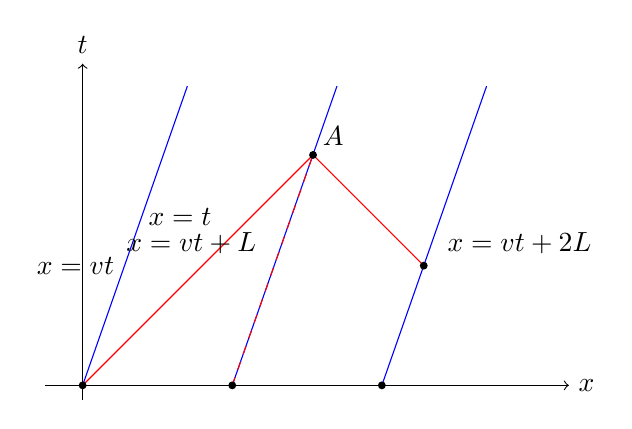
\begin{tikzpicture}[scale=0.95]
\draw[->] (-0.5,0) -- (6.5,0) node[right] {$x$};
\draw[->] (0,-0.2) -- (0,4.3) node[above] {$t$};

\draw[blue] (0,0) -- (1.4,4.0);
\draw[blue] (2.0,0) -- (3.4,4.0);
\draw[blue] (4.0,0) -- (5.4,4.0);

\draw[red] (0,0) -- (3.08,3.08);
\draw[red] (3.08,3.08) -- (4.56,1.60);
\draw[red,dashed] (2.0,0) -- (3.08,3.08);

\fill (0,0) circle (1.5pt);
\fill (2.0,0) circle (1.5pt);
\fill (4.0,0) circle (1.5pt);
\fill (3.08,3.08) circle (1.5pt);
\fill (4.56,1.60) circle (1.5pt);

\node[left] at (0.55,1.6) {$x=vt$};
\node[left] at (2.45,1.9) {$x=vt+L$};
\node[right] at (4.75,1.9) {$x=vt+2L$};
\node[left] at (1.85,2.25) {$x=t$};
\node[above right] at (3.08,3.08) {$A$};
\end{tikzpicture}
\caption{Reconstruction of the simultaneity argument. The screenshot preserves the board logic; the redraw makes the equations explicit.}
\end{figure}

\paragraph{Worked derivation.} The key intermediate point is the point \(A\) where the forward light ray \(x=t\) meets the shifted worldline \(x=vt+L\). Its coordinates are obtained by solving
\begin{align}
x &= t, \\
x &= vt+L.
\end{align}
Substituting \(x=t\) into the second equation,
\begin{equation}
t=vt+L,
\end{equation}
so
\begin{equation}
(1-v)t=L,
\end{equation}
and therefore
\begin{equation}
t_A=\frac{L}{1-v},\qquad x_A=\frac{L}{1-v}.
\end{equation}

Now we trace a backward-going light ray from \(A\). Such a ray has the form
\begin{equation}
x=-t+b,
\end{equation}
or equivalently
\begin{equation}
x+t=b.
\end{equation}
To determine \(b\), we use the fact that the ray passes through \(A\). At \(A\), \(x=t=L/(1-v)\), so
\begin{equation}
b=x_A+t_A=\frac{2L}{1-v}.
\end{equation}
Hence the backward light ray is
\begin{equation}
x+t=\frac{2L}{1-v}.
\end{equation}

The point we really want is where this backward light ray hits the next shifted worldline \(x=vt+2L\). So we solve
\begin{align}
x+t &= \frac{2L}{1-v}, \\
x &= vt+2L.
\end{align}
Substituting the second equation into the first gives
\begin{equation}
vt+2L+t=\frac{2L}{1-v}.
\end{equation}
Rearranging,
\begin{equation}
(1+v)t=2L\left(\frac{1}{1-v}-1\right)=2L\frac{v}{1-v},
\end{equation}
and so
\begin{equation}
t=\frac{2Lv}{1-v^2}.
\end{equation}
Substituting back,
\begin{equation}
x=vt+2L=\frac{2L}{1-v^2}.
\end{equation}
The slope of the simultaneity line is therefore
\begin{equation}
\frac{t}{x}=v,
\end{equation}
which means that the moving observer's line of simultaneity through the origin is
\begin{equation}
t=vx.
\end{equation}

This is the geometric heart of the lecture. The moving time axis is the line
\begin{equation}
x=vt,
\end{equation}
while the moving line of simultaneity is
\begin{equation}
t=vx.
\end{equation}
The two are tilted symmetrically with respect to the \(45^\circ\) light rays.

When we restore dimensions, only one form is possible:
\begin{equation}
t=\frac{v}{c^2}x.
\end{equation}
For ordinary velocities this slope is tiny, which is why the relativity of simultaneity is usually invisible in daily experience.

\section{From Tilted Axes to the Lorentz Transformation}

Once the geometry has been extracted, Susskind redraws it in a cleaner, more symmetric form. The board picture matters here because the symmetry is part of the argument, not merely a decoration.

\begin{figure}
\centering

\includegraphics[width=0.72\textwidth]{lecture_01_figure_05.png}
\caption{Symmetric \(c=1\) spacetime diagram.}
\end{figure}

\begin{figure}
\centering
\begin{tikzpicture}[scale=1.0]
\draw[->] (-2.2,0) -- (5.2,0) node[right] {$x$};
\draw[->] (0,-0.2) -- (0,4.9) node[above] {$t$};

\draw[red] (0,0) -- (3.9,3.9);
\draw[red] (0,0) -- (-1.8,1.8);

\draw[blue] (0,0) -- (1.8,4.5);
\draw[blue,dashed] (0,0) -- (4.5,1.8);

\node[right] at (3.9,3.9) {$x=t$};
\node[left] at (-1.8,1.8) {$x=-t$};
\node[above] at (1.8,4.5) {$x'=0$};
\node[right] at (4.5,1.8) {$t'=0$};
\end{tikzpicture}
\caption{Cleaned \(c=1\) diagram showing the primed time axis, the primed simultaneity axis, and the two light rays.}
\end{figure}

In the lecture the notation on the board shifts later to uppercase \(X\) and \(T\), but the content is unchanged. We keep the lower-case notation \(x,t\) throughout.

The geometry already tells us the zero-sets of the new coordinates. Since the moving origin is the line \(x=vt\), the equation for \(x'\) must vanish there. That suggests the linear form
\begin{equation}
x'=\frac{x-vt}{F(v)}.
\end{equation}
Likewise the moving line of simultaneity is the line \(t=vx\), and along that line we want \(t'=0\). So we write
\begin{equation}
t'=\frac{t-vx}{G(v)}.
\end{equation}
At this stage \(F(v)\) and \(G(v)\) are unknown denominator functions.

Now use the invariance of light speed. If a light ray satisfies \(x=t\), then it must also satisfy \(x'=t'\). Substituting \(x=t\) into the two expressions gives
\begin{align}
x' &= \frac{(1-v)t}{F(v)}, \\
t' &= \frac{(1-v)t}{G(v)}.
\end{align}
For these to be equal along every light ray of this form, we must have
\begin{equation}
F(v)=G(v).
\end{equation}
So the transformation becomes
\begin{equation}
x'=\frac{x-vt}{F(v)},\qquad t'=\frac{t-vx}{F(v)}.
\end{equation}

We still need \(F(v)\). Multiply through by \(F(v)\):
\begin{align}
F(v)x' &= x-vt, \\
F(v)t' &= t-vx.
\end{align}
To solve for \(x\), multiply the second equation by \(v\) and add it to the first. The \(vt\) terms cancel, leaving
\begin{equation}
(1-v^2)x=F(v)\bigl(x'+vt'\bigr).
\end{equation}
Thus
\begin{equation}
x=\frac{F(v)\bigl(x'+vt'\bigr)}{1-v^2}.
\end{equation}
By the same method,
\begin{equation}
t=\frac{F(v)\bigl(t'+vx'\bigr)}{1-v^2}.
\end{equation}

Now comes the final physical input: reciprocity. The inverse transformation should have the same form as the forward transformation, except that the sign of the relative velocity reverses. That requires
\begin{equation}
\frac{F(v)}{1-v^2}=\frac{1}{F(v)}.
\end{equation}
Multiplying through by \(F(v)\), we find
\begin{equation}
F(v)^2=1-v^2,
\end{equation}
and therefore
\begin{equation}
F(v)=\sqrt{1-v^2}.
\end{equation}
Because \(F(v)\) appears in the denominator, this is exactly the lecture's convention: the denominator is \(\sqrt{1-v^2}\).

We have arrived at the Lorentz transformation in units with \(c=1\):
\begin{align}
x' &= \frac{x-vt}{\sqrt{1-v^2}}, \\
t' &= \frac{t-vx}{\sqrt{1-v^2}}.
\end{align}
The inverse relations are
\begin{align}
x &= \frac{x'+vt'}{\sqrt{1-v^2}}, \\
t &= \frac{t'+vx'}{\sqrt{1-v^2}}.
\end{align}

To restore dimensions, we replace \(v^2\) by \(v^2/c^2\), and in the time equation we insert the necessary factor of \(1/c^2\):
\begin{align}
x' &= \frac{x-vt}{\sqrt{1-v^2/c^2}}, \\
t' &= \frac{t-(v/c^2)x}{\sqrt{1-v^2/c^2}}.
\end{align}
If one later introduces
\begin{equation}
\gamma=\frac{1}{\sqrt{1-v^2/c^2}},
\end{equation}
these become the familiar textbook formulas. But the lecture reaches them first in the denominator form, and that order is worth preserving.

\paragraph{A direct check.} The lecture ends by checking the formulas on a light ray. If
\begin{equation}
x=ct,
\end{equation}
then
\begin{align}
x' &= \frac{(c-v)t}{\sqrt{1-v^2/c^2}}, \\
t' &= \frac{(1-v/c)t}{\sqrt{1-v^2/c^2}}.
\end{align}
Therefore
\begin{equation}
\frac{x'}{t'}=\frac{c-v}{1-v/c}=c.
\end{equation}
So a right-moving light ray still moves with speed \(c\) in the primed frame. The same calculation shows that \(x=-ct\) becomes \(x'=-ct'\) for a left-moving light ray.

There is also an important limiting check. When \(v\ll c\), both \(v^2/c^2\) and \((v/c^2)x\) are negligible in ordinary circumstances. Then the Lorentz transformation reduces approximately to
\begin{equation}
t'\approx t,\qquad x'\approx x-vt,
\end{equation}
which is exactly Galileo's transformation. The Galilean world was not false in its own domain; it was incomplete.

The truly new statement is not merely that \(x\) transforms differently, but that the families \(t=\text{constant}\) and \(t'=\text{constant}\) are different families. What is simultaneous in one inertial frame is not simultaneous in another.

\section{Summary}

The lecture begins with a frame of reference understood operationally as a lattice of meter sticks and synchronized clocks. From that picture one reads off the Galilean transformation and then tests it. Simultaneous separation is invariant, velocity is not, acceleration is, and that is why Newtonian mechanics naturally takes the form \(F=ma\).

The lecture then turns to the clash with electromagnetism. Galilean kinematics predicts that a moving observer sees light at speed \(c-v\), while Einstein insists that light has the same speed in every inertial frame. That forces a return to first principles, especially the synchronization of distant clocks by light signals. The result is the relativity of simultaneity.

From the concrete light-signal construction one finds the moving time axis \(x=vt\) and the moving simultaneity axis \(t=vx\) in \(c=1\) units. From that geometry, plus light-speed invariance and reciprocity, one obtains the Lorentz transformation. The lecture stops there, with the central lesson already in hand: time is not a universal background parameter. Next come the consequences of this fact, especially length contraction, time dilation, and the rest of relativistic kinematics.